\chapter{Introduction}
\label{chap:aChapter}
\begin{flushright}{\slshape    
   Science, my boy, is made up of mistakes, but they are mistakes
   which it is useful to make, because they lead little by little
   to the truth}. \\ \medskip --- \citeauthor{verne_journey:1957}
   \citetitle{verne_journey:1957}
\end{flushright} 

This template is ready to be used when writing a thesis at
\myDepartment. It is a modified version of Classic Thesis by
Andr\'e Miede that can be found here
\url{http://code.google.com/p/classicthesis/}. Refer to its manual
for further informations. Any other package included have also its
own manual that can be found by searching its name on Internet.
Additional hints in italian can be found in \enquote{Introduzione
allo stile Classic Thesis} and more general ones in \enquote{L'arte di
scrivere con latex} both by Lorenzo Pantieri. If none of these
answer your question, ask it on
\url{http://tex.stackexchange.com/}.

\section{Showcase}
Usefull features of the template are shown and explained.

\subsection{File structure}
The template is organized in multiple files. In the root folder,
the main file which is to be compiled is
\verb!ClassicThesis_DEIB.tex!. You should just add the source
files you want to include and any hyphenation you need to
explictly specify. The \verb!classicthesis-config.tex! contains
options that can be chosen for this template. It contains also
the definition for the title, the author and others stuff
displayed in the titlepage. It is commented enough to be used.
The other file present is \verb!Bibliography.bib! which is the
\emph{Bibtex} database.

The other folders are:
\begin{aenumerate}
	\item \verb!Chapters! contains source files for the main chapters
	of your thesis;
	\item \verb!CodeFiles! contains any code snippet you want to
	include in your thesis with the environment \verb!listings!;
	\item \verb!FrontBackmatter! contains various files that are
	included to produce abstract, titlepages, acknoledgements,
	\ldots. Modify them with your informations;
	\item \verb!Images! contains the \verb!.pdf! or \verb!.png!
	versions of the images of the thesis. A \verb!sources! subfolder
	is also provided for keeping the original Inkscape, GIMP,
	Photoshop or whatever you use.
\end{aenumerate}

\subsection{Environments}
In addition to common \LaTeX\ environments, this thesis is set to
use:
\begin{itemize}
	\graffito{The command graffito is used to put some text here,
	usefull to underline important things in long paragraphs.}
	\item \verb!\begin{aenumerate}! to produce an \verb!\enumerate!
	with letters instead of numbers, as above;
	\item \verb!\blockcquote[][]{}{}! to
	\blockcquote[see][p. 111]{bringhurst:2002}{produce a citation
	with reference to author and page}. If the citation is longer
	than two rows is indented. This is provided by package
	\verb!csquotes!, which settings are in
	\verb!classicthesis-config.tex!. The package also provides
	\verb!\enquote{citation}! that produces \enquote{correct citation
	style} according to the language in use.
	\item \verb!\ac{}! and its variations, defined by package
	\verb!acronyms!, provide nice handling for acronyms, like
	\ac{XML}. They are listed after figures and tables before the
	abstract.
	\item the so called semi-dynamic referencing for chapter,
	sections, figures, etc. A set of command like
	\verb!\myChap{label_key}! are provided to produce things like
	\myChap{chap:aChapter}. There are also capital versions of the
	commands (\verb!\MyChap{}! produces \MyChap{chap:aChapter}) and
	commands for equations (\verb!\myEq{}! produces
	\myEq{eq:massConservation}).
	\item references to bibliography are produced in the usual way
	with \verb!\cite{bib_key}! \cite{bringhurst:2002} and its
	variations \verb!\citeauthor{bib_key}!,
	\verb!\citetitle{bib_key}! and others.
	\item figures are handled usually with the code
	\begin{verbatim}
	\begin{figure}
	\centering
	\includegraphics[width=\columnwidth]{Images/name.pdf} 
	\caption[Short description]{Long description.}
	\label{fig:massConstraintFeasibility}
	\end{figure}
	\end{verbatim}
	which produces \myFig{fig:massConstraintFeasibility}.
	\item tables are produced with
	\begin{verbatim}
	\begin{table}[tb]
	\footnotesize
	\centering
	\begin{tabularx}{0.8\textwidth}{llrcl}
	\toprule
	\tableheadline{l}{Algorithm} &
	\tableheadline{l}{Parameter} &
	\tableheadlineMore{3}{c}{Suggested Values} \\
	\midrule
	\tablefirstcol{l}{Any}
	& \acs{NFE} 		& $10\,000 $ & $ \div $ & $ 200\,000$ \\
	& Population Size 	&  $10 $ & $ \div 	$ & $ 1000$ \\
	\midrule
	\tablefirstcol{l}{\ac{GDE3}}
	& \ac{DE} step size & $0.0 $ & $\div $ & $ 1.0$ \\
	& Crossover rate 	& $0.0$ & $ \div $ & $ 1.0$ \\
	\bottomrule
	\end{tabularx}
	\caption[Short description]{Long description.}
	\label{tab:MOEAandParameters}
	\end{table}
	\end{verbatim}
    which produces \myTab{tab:MOEAandParameters}.
    \verb!\myfloatalign!, \verb!\tableheadline{}{}! and its
    variation \verb!\tableheadlineMore{}{}{}! and
    \verb!\tablefirstcol{}{}! are used to give a common style to
    all tables in the document. They are defined in
    \verb!classicthesis-config.tex!.\footnote{Also do not forget
    footnotes, which should be placed after the punctuation mark.}
\end{itemize}

\begin{equation}
\nabla \mathbf{q_s} = U(x,y) - b_t
\label{eq:massConservation}
\end{equation}

\begin{figure}
\centering
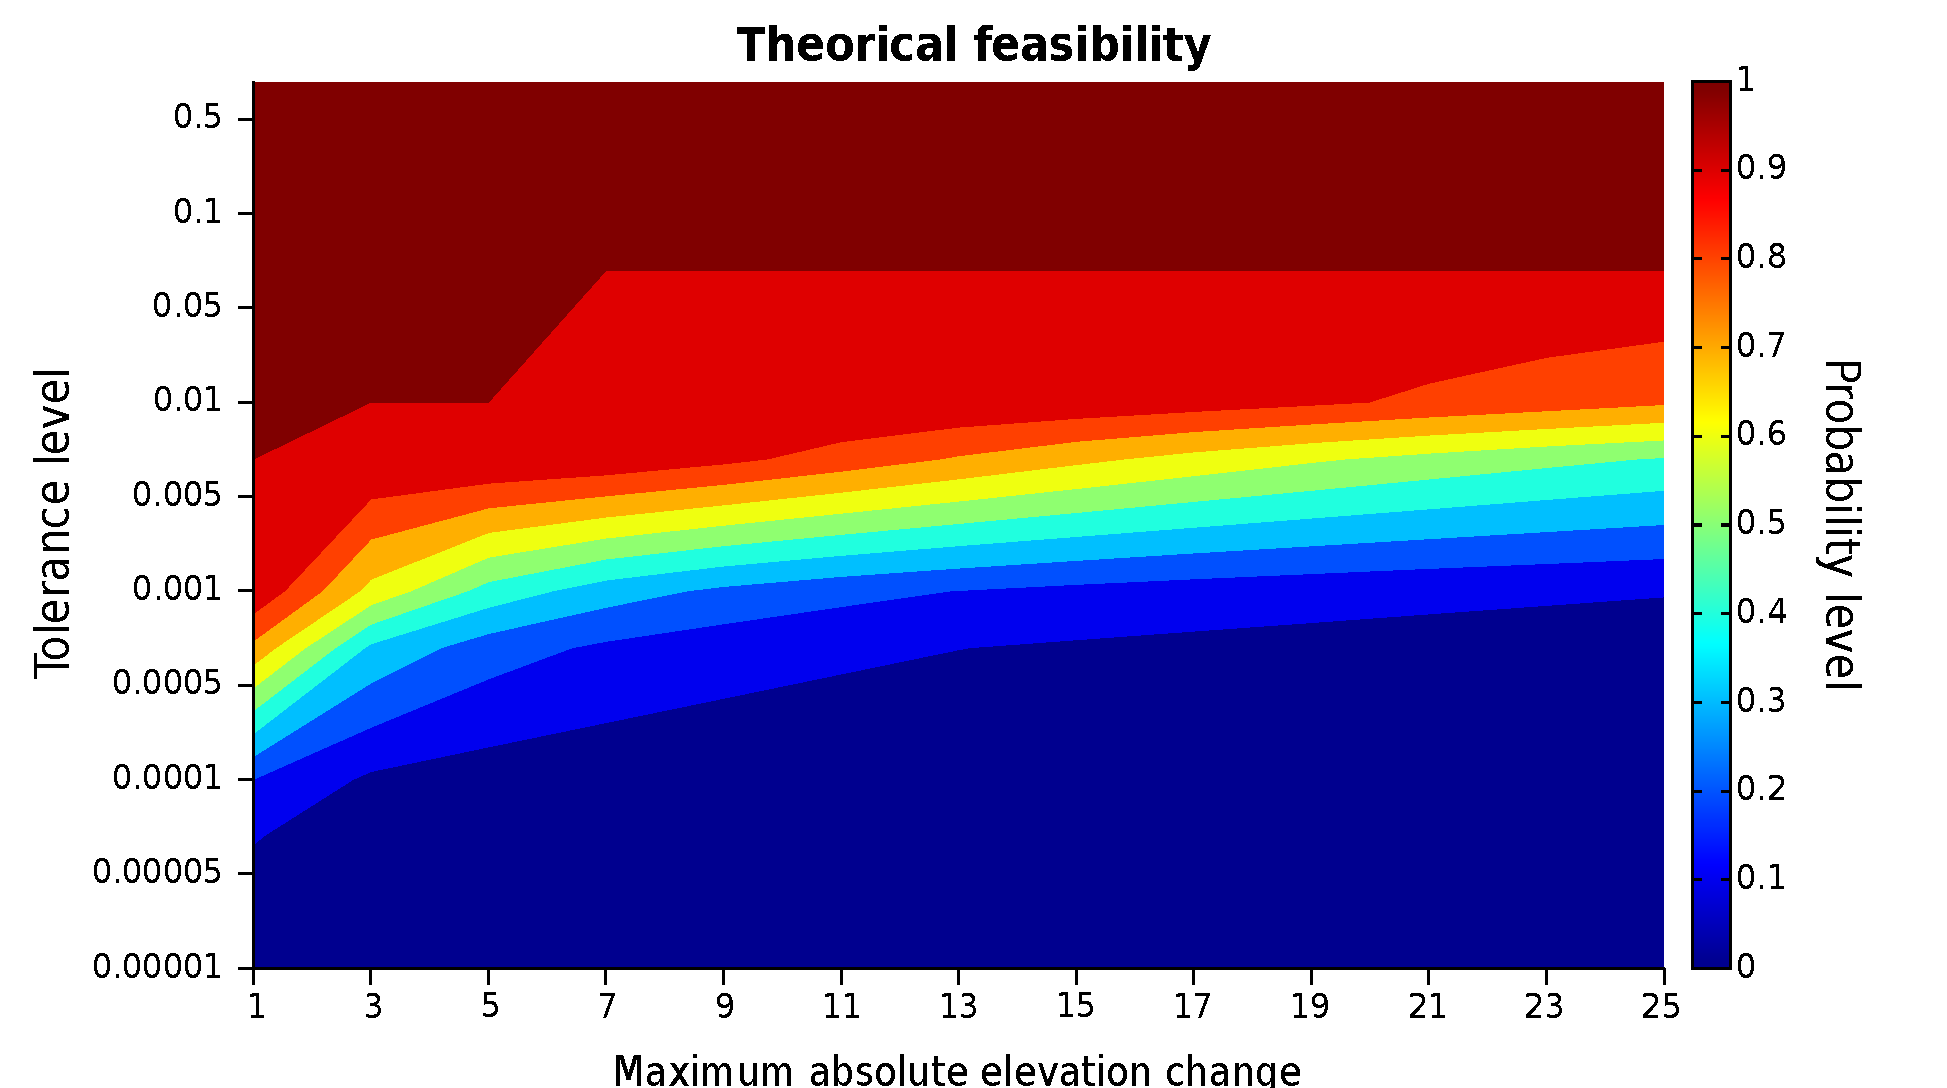
\includegraphics[width=\columnwidth]{Images/feasibilityNR51.pdf}  
\caption[Theoretical probability of randomly choose a surface
respecting the \ac{DEM} elevations sum constraint]{Theoretical
probability of randomly choose a surface respecting the \ac{DEM}
elevations sum constraint: the blue area represents low
probabilities, the red higher ones. On the $y$-axis there is the
tolerance on the accepted mass variation. On the $x$-axis there is
the range of possible variations in meters, \eg $5$ means that
each cell can vary from its initial condition of $\pm 5$ meters.
\acs{DEM} dimensions are $51 \times 51$.}
\label{fig:massConstraintFeasibility}
\end{figure}

\begin{table}
\footnotesize
\centering
\begin{tabularx}{0.8\textwidth}{llrcl}
\toprule
\tableheadline{l}{Algorithm} &
\tableheadline{l}{Parameter} &
\tableheadlineMore{3}{c}{Suggested Values} \\
\midrule
\tablefirstcol{l}{Any}
& \acs{NFE} 		& $10\,000 $ & $ \div $ & $ 200\,000$ \\
& Population Size 	&  $10 $ & $ \div 	$ & $ 1000$ \\
\midrule
\tablefirstcol{l}{\ac{GDE3}}
& \ac{DE} step size & $0.0 $ & $\div $ & $ 1.0$ \\
& Crossover rate 	& $0.0$ & $ \div $ & $ 1.0$ \\
\bottomrule
\end{tabularx}
\caption[Parameters needed for each \ac{MOEA} used]{Parameters
needed for each \ac{MOEA} used: if the algorithm requires the
parameter, a range is given as in literature.}
\label{tab:MOEAandParameters}
\end{table}

These are the main commands used: others are missing and many can
be improved or refined. Suggestion are welcome at
\url{http://code.google.com/p/}
